% 18 variables in here:
% h_1 = 10.0, h_2 = 11.0, h_3 = 11.0, h_4 = 11.0, h_5 = 11.0, h_6 = 11.0, ux_1 = 0.0, ux_2 = 0.0, ux_3 = 0.0, ux_4 = 0.0, ux_5 = 0.0, ux_6 = 0.0, uy_1 = 0.0, uy_2 = 0.0, uy_3 = 0.0, uy_4 = 0.0, uy_5 = 0.0, uy_6 = 0.0
\begin{figure}[h!]
\centering
  \subfigure[1st basis function, $x$-momentum -- 1st basis function, $y$-momentum] {
    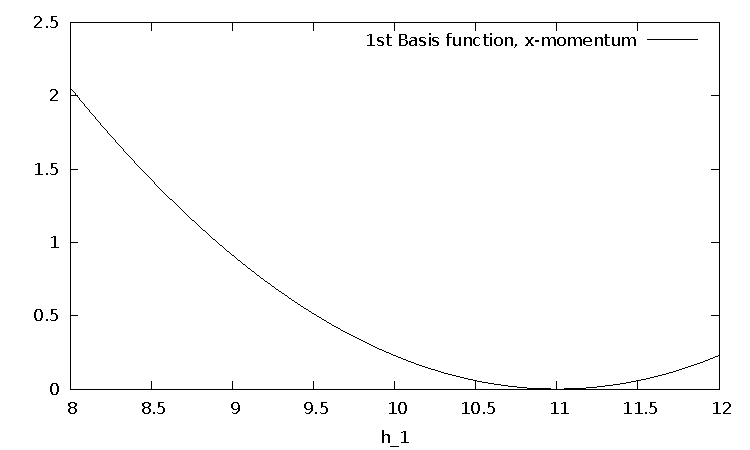
\includegraphics[scale=\zoomfactor]{{{ord2_varying_h1_h2-h6_11/y_11.0_11.0_11.0_11.0_11.0_0.0_0.0_0.0_0.0_0.0_0.0_0.0_0.0_0.0_0.0_0.0_0.0f00}}}
  }
  % \subfigure[] {
  %   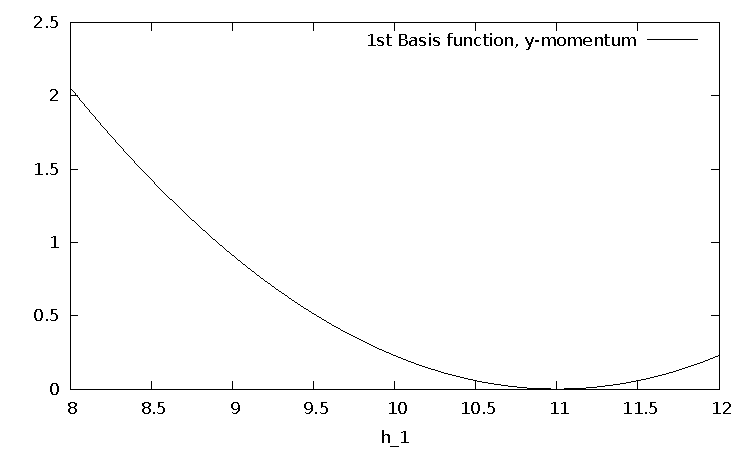
\includegraphics[scale=\zoomfactor]{{{ord2_varying_h1_h2-h6_11/y_11.0_11.0_11.0_11.0_11.0_0.0_0.0_0.0_0.0_0.0_0.0_0.0_0.0_0.0_0.0_0.0_0.0f01}}}
  % }
  \subfigure[2nd basis function, $x$-momentum -- 6th basis function, $y$-momentum] {
    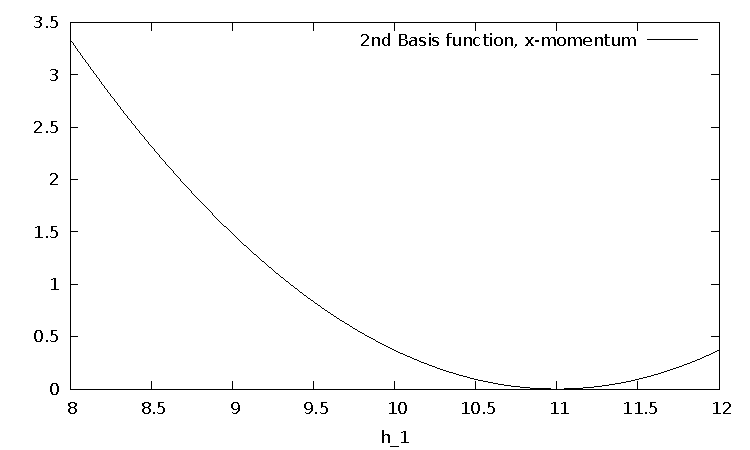
\includegraphics[scale=\zoomfactor]{{{ord2_varying_h1_h2-h6_11/y_11.0_11.0_11.0_11.0_11.0_0.0_0.0_0.0_0.0_0.0_0.0_0.0_0.0_0.0_0.0_0.0_0.0f02}}}
  }
  \subfigure[2nd basis function, $y$-momentum -- 4th basis function, $x$-momentum -- 4th basis function, $y$-momentum -- 6th basis function, $x$-momentum] {
    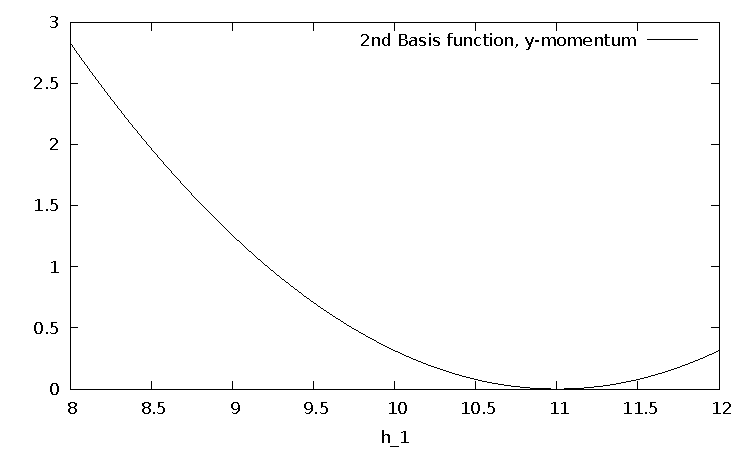
\includegraphics[scale=\zoomfactor]{{{ord2_varying_h1_h2-h6_11/y_11.0_11.0_11.0_11.0_11.0_0.0_0.0_0.0_0.0_0.0_0.0_0.0_0.0_0.0_0.0_0.0_0.0f03}}}
  }
  \subfigure[3rd basis function, $x$-momentum -- 5th basis function, $y$-momentum] {
    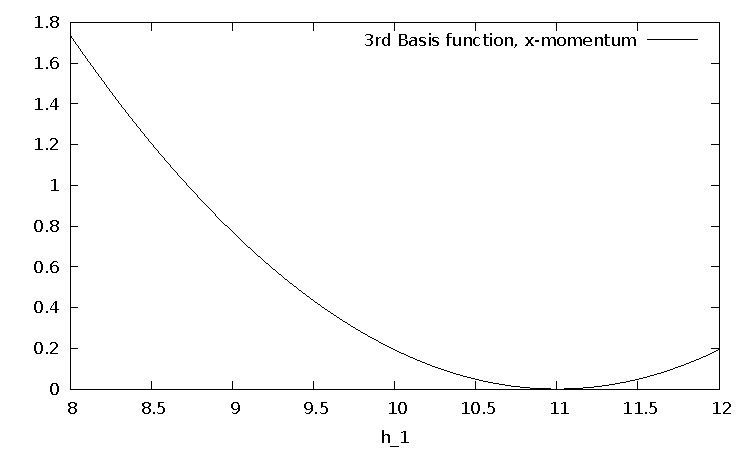
\includegraphics[scale=\zoomfactor]{{{ord2_varying_h1_h2-h6_11/y_11.0_11.0_11.0_11.0_11.0_0.0_0.0_0.0_0.0_0.0_0.0_0.0_0.0_0.0_0.0_0.0_0.0f04}}}
  }
  % \subfigure[3rd basis function, $y$-momentum -- 5th basis function, $x$-momentum] {
  %   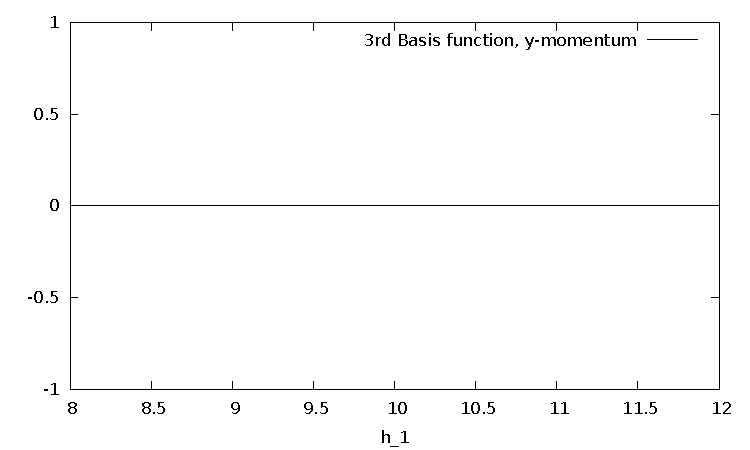
\includegraphics[scale=\zoomfactor]{{{ord2_varying_h1_h2-h6_11/y_11.0_11.0_11.0_11.0_11.0_0.0_0.0_0.0_0.0_0.0_0.0_0.0_0.0_0.0_0.0_0.0_0.0f05}}}
  % }
  % \subfigure[] {
  %   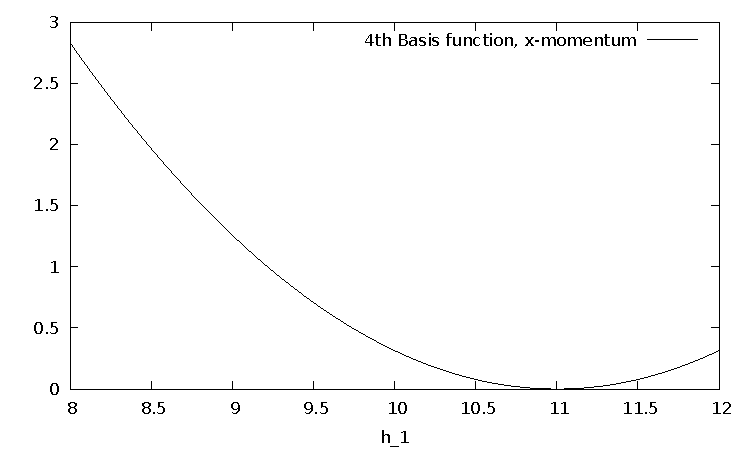
\includegraphics[scale=\zoomfactor]{{{ord2_varying_h1_h2-h6_11/y_11.0_11.0_11.0_11.0_11.0_0.0_0.0_0.0_0.0_0.0_0.0_0.0_0.0_0.0_0.0_0.0_0.0f06}}}
  % }
  % \subfigure[] {
  %   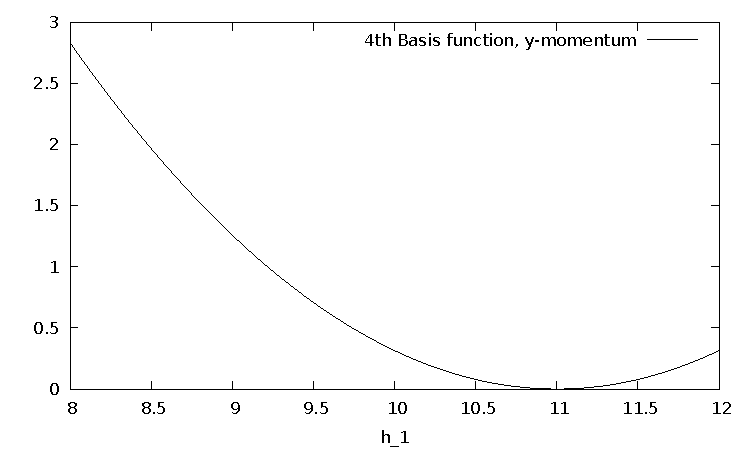
\includegraphics[scale=\zoomfactor]{{{ord2_varying_h1_h2-h6_11/y_11.0_11.0_11.0_11.0_11.0_0.0_0.0_0.0_0.0_0.0_0.0_0.0_0.0_0.0_0.0_0.0_0.0f07}}}
  % }
  % \subfigure[] {
  %   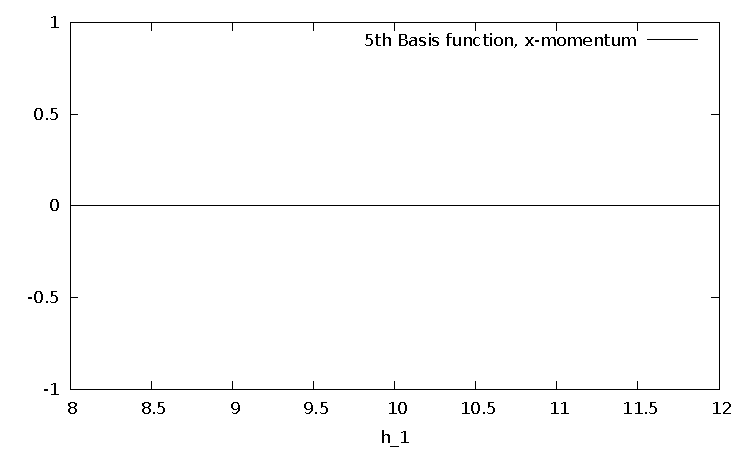
\includegraphics[scale=\zoomfactor]{{{ord2_varying_h1_h2-h6_11/y_11.0_11.0_11.0_11.0_11.0_0.0_0.0_0.0_0.0_0.0_0.0_0.0_0.0_0.0_0.0_0.0_0.0f08}}}
  % }
  % \subfigure[] {
  %   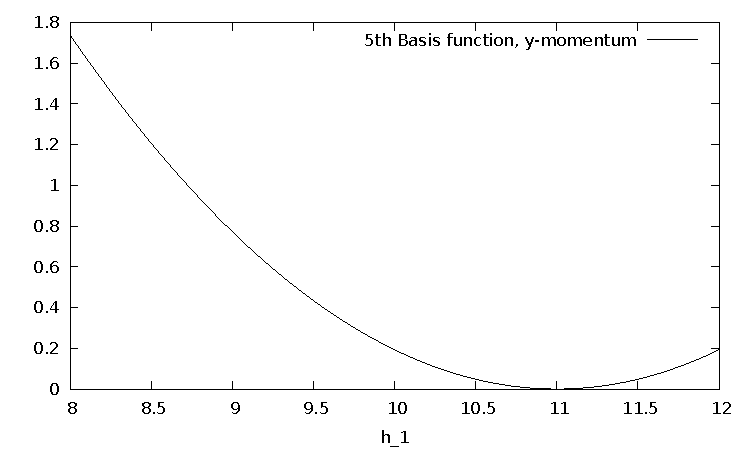
\includegraphics[scale=\zoomfactor]{{{ord2_varying_h1_h2-h6_11/y_11.0_11.0_11.0_11.0_11.0_0.0_0.0_0.0_0.0_0.0_0.0_0.0_0.0_0.0_0.0_0.0_0.0f09}}}
  % }height 
  % \subfigure[] {
  %   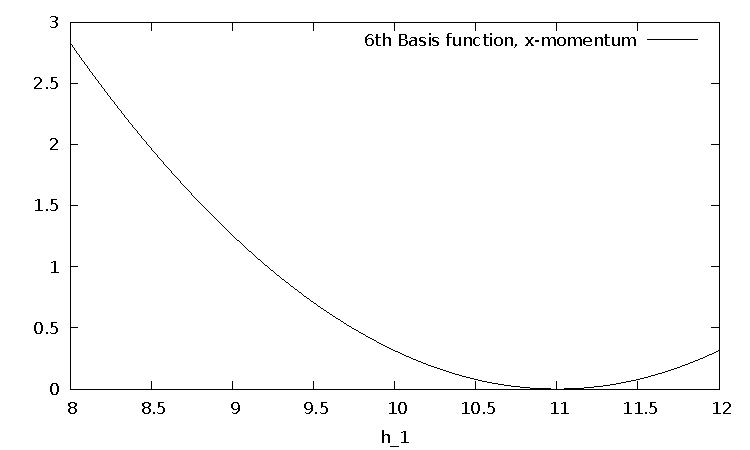
\includegraphics[scale=\zoomfactor]{{{ord2_varying_h1_h2-h6_11/y_11.0_11.0_11.0_11.0_11.0_0.0_0.0_0.0_0.0_0.0_0.0_0.0_0.0_0.0_0.0_0.0_0.0f10}}}
  % }
  % \subfigure[] {
  %   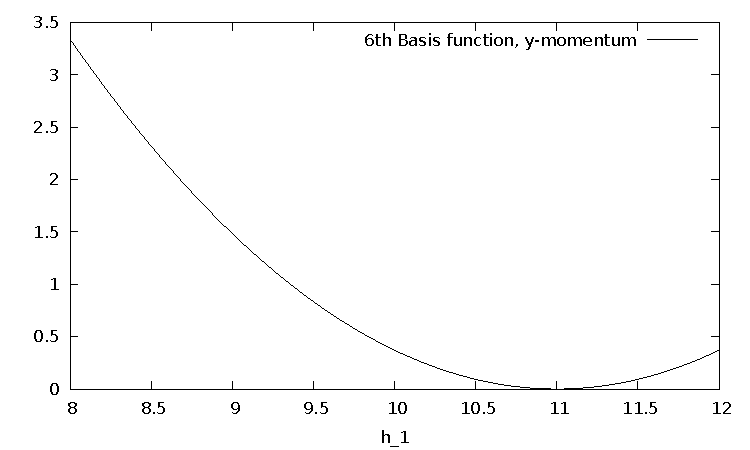
\includegraphics[scale=\zoomfactor]{{{ord2_varying_h1_h2-h6_11/y_11.0_11.0_11.0_11.0_11.0_0.0_0.0_0.0_0.0_0.0_0.0_0.0_0.0_0.0_0.0_0.0_0.0f11}}}
  % }
\caption{Error plots for varying $h_1$. All heights $h_2$ to $h_6$ are fixed to 11. All momentums are 0. Note that the error is always minimal for $h_1=11$. The errors for the $y$-momentum of the 3rd basis function and the $x$-momentum of the 5th basis function are zero.}
\label{fig:ord2_varying_h1_h2-h6_11}
\end{figure}

%%% Local Variables:
%%% TeX-master: "../results.tex"
%%% End:
